\begin{figure}[H]
    \centering
    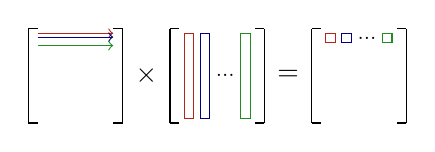
\begin{tikzpicture}[scale=1.2]
        \draw (-1.25,-0.5) -- (-1.25,0.5);
        \draw (-1.25,-0.5) -- (-1.15,-0.5);
        \draw (-1.25,0.5) -- (-1.15,0.5);
        \draw (-0.25,-0.5) -- (-0.25,0.5);
        \draw (-0.25,-0.5) -- (-0.35,-0.5);
        \draw (-0.25,0.5) -- (-0.35,0.5);

        \node at (0,0) () {$\times$}; 

        \draw (1.25,-0.5) -- (1.25,0.5);
        \draw (1.25,-0.5) -- (1.15,-0.5);
        \draw (1.25,0.5) -- (1.15,0.5);
        \draw (0.25,-0.5) -- (0.25,0.5);
        \draw (0.25,-0.5) -- (0.35,-0.5);
        \draw (0.25,0.5) -- (0.35,0.5);

        \node at (1.5,0) () {$=$};

        \draw (2.75,-0.5) -- (2.75,0.5);
        \draw (2.75,-0.5) -- (2.65,-0.5);
        \draw (2.75,0.5) -- (2.65,0.5);
        \draw (1.75,-0.5) -- (1.75,0.5);
        \draw (1.75,-0.5) -- (1.85,-0.5);
        \draw (1.75,0.5) -- (1.85,0.5);

        \draw[color=BrickRed, ->] (-1.15,0.45) -- (-0.35,0.45);
        \draw[color=NavyBlue, ->] (-1.15,0.41) -- (-0.35,0.41);
        \node at (0.835,0) () {\scriptsize{...}};
        \draw[color=ForestGreen, ->] (-1.15,0.32) -- (-0.35,0.32);

        \draw[color=BrickRed] (0.4,-0.45) rectangle (0.5,0.45);
        \draw[color=NavyBlue] (0.57,-0.45) rectangle (0.67,0.45);
        \draw[color=ForestGreen] (1,-0.45) rectangle (1.1,0.45);

        \draw[color=BrickRed] (1.9,0.35) rectangle (2,0.45);
        \draw[color=NavyBlue] (2.07,0.35) rectangle (2.17,0.45);
        \node at (2.335,0.4) () {\scriptsize{...}};
        \draw[color=ForestGreen] (2.5,0.35) rectangle (2.6,0.45);
    \end{tikzpicture}
\end{figure}